\setcounter{section}{6}

\Needspace{5\baselineskip}
\hypertarget{dueling-dqn}{%
\section{Dueling DQN}\label{dueling-dqn}}

DQN中，\(Q\) 是一个同时由状态 \(s\) 和动作 \(a\) 决定的函数。但在某些状态下，智能体只需要知道``现在的环境好不好''（\(V\) 值），而不关心具体动作的差异；而在需要通过做动作来避险或得分时，才需要关心``哪个动作比平均水平好''（\(A\) 值）。如果我们将两者分开建模，\(V(s)\) 专门负责看大局，评估当前环境好不好；\(A(s,a)\) 专门负责看细节，评估在当前环境下，哪个动作比其他动作好，好多少。这种解耦使得 \(V(s)\) 可以在每一个样本中都被学习更新（因为无论选哪个动作，\(V(s)\) 都是基础），从而大幅提升了训练效率。

\begin{figure}[htbp]
\centering
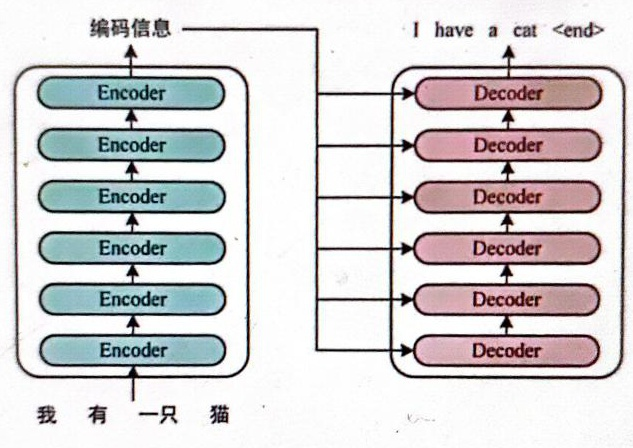
\includegraphics{images/image-0015.jpeg}
\caption{Dueling DQN 中状态价值和动作优势的直观区别}
\end{figure}

场景 A（大直道，前方无车）：此时通过屏幕（状态 \(s\)），可以判断当前局势较稳，在这个状态下大概率能得高分。此时，无论稍微向左打方向盘，还是向右打方向盘（动作 \(a\)），对最终得分的影响都较小。

\begin{itemize}
\tightlist
\item
  结论：此时 \(V(s)\)（状态价值）很高，而 \(A(s,a)\)（动作优势）的差异很小。神经网络不必费力学习每个动作的具体数值，只需要知道``这里不错''即可。
\end{itemize}

场景 B（前方有障碍物，必须急转弯）：此时状态 \(s\) 很危险，如果不操作好就会撞车。

\begin{itemize}
\tightlist
\item
  结论：此时动作选择非常重要，向左转可能存活，向右转可能失败。这时 \(A(s,a)\)（动作优势）的差异很大。
\Needspace{5\baselineskip}
  从而我们把Q函数拆分如下：
\end{itemize}

\[
Q(s,a;\theta,\alpha,\beta)=V(s;\theta,\beta)+A(s,a;\theta,\alpha)
\]

\begin{itemize}
\tightlist
\item
  \(\theta\)：共享参数（卷积层），负责从图像中提取边缘、形状、物体位置等通用特征。这些特征既对判断局势有用，也对选择动作有用。
\item
  \(\beta\)：价值流参数（全连接层），将特征映射为一个标量 \(V\)。
\item
  \(\alpha\)：优势流参数（全连接层），将特征映射为一个向量 \(A\)，维度为动作数。
  但问题在于，我们计算和更新的都是 \(Q\) 值，怎么从 \(Q\) 值中求出 \(V\) 和 \(A\)？
\end{itemize}

\Needspace{5\baselineskip}
我们可以获取同一个状态 \(s\) 上的所有动作 \(a'\)（遍历），各个动作 \(Q\) 值的相对大小关系也就是它们的 \(A\) 值相对大小。一个方案是对于给定 \(s\)，取让 \(Q(s,a')\) 最大的动作 \(a^*\)，设 \(A(s,a^*)=0\)（最大动作优势值），\(V(s)=Q(s,a^*)\)，则：

方案 A：Max 约束（理论最优）

\[
Q(s,a)=V(s)+(A(s,a)-\max_{a'}A(s,a'))
\]

\begin{itemize}
\tightlist
\item
  数学含义：强制让最大的优势值为 \(0\)。
\Needspace{5\baselineskip}
  另一方案是取所有动作优势值的平均值为0：
\end{itemize}

方案 B：Mean 约束（工程最优）

\[
Q(s,a)=V(s)+(A(s,a)-\frac{1}{|\mathcal{A}|}\sum_{a'}A(s,a'))
\]

\begin{itemize}
\item
  数学含义：强制让所有动作的优势值之和为 \(0\)，也就是平均值为 \(0\)。
\item
  为什么更好：\(\max\) 操作是非线性操作，梯度只在最大值处传递，其他位置梯度为 \(0\)；而 mean 操作涉及所有动作的求和，梯度可以平滑地回传给每一个动作优势输出节点。
\item
  抗噪性：均值对异常值不那么敏感，能让网络训练更平稳。
\Needspace{5\baselineskip}
  这样虽然不严格满足贝尔曼最优方程，但在工程实现上更优。原因如下：
\item
  数学含义：强制让所有动作的优势值之和为 \(0\)（即平均值为 \(0\)）。
\item
\Needspace{5\baselineskip}
  为什么更好：

  \begin{itemize}
  \tightlist
  \item
    梯度稳定性：\(\max\) 操作是一个非线性操作，梯度只在最大值处传递，其他位置梯度为 \(0\)。而 mean 操作涉及所有动作的求和，梯度可以平滑地回传给每一个动作的优势输出节点。
  \item
    抗噪性：均值对异常值不那么敏感，能让网络训练更平稳。
  \end{itemize}
\end{itemize}

\FloatBarrier
\Needspace{5\baselineskip}
\hypertarget{ux53c2ux8003ux6587ux732e-52}{%
\subsection{参考文献}\label{ux53c2ux8003ux6587ux732e-52}}

\vspace{0.25em}
\begin{itemize}
\tightlist
\item
  Wang, Z., Schaul, T., Hessel, M., van Hasselt, H., Lanctot, M., \& de Freitas, N. (2016). \href{https://arxiv.org/abs/1511.06581}{Dueling Network Architectures for Deep Reinforcement Learning}. ICML 2016.
\item
  \href{https://hrl.boyuai.com/}{《动手学强化学习》}.
\end{itemize}

\clearpage
